% Chapter 5: YOLO Architecture and Training Strategies
% IEEE-style comprehensive textbook chapter


\section{Introduction}

The You Only Look Once (YOLO) family of object detection algorithms has revolutionized real-time computer vision applications through its unified approach to detection, treating object localization and classification as a single regression problem rather than a pipeline of separate components. This chapter provides a comprehensive examination of YOLO architecture evolution, model selection considerations for synthetic data training scenarios, and training configurations optimized for reinforcement learning feedback loops. The integration of YOLO detectors within synthetic-to-real domain adaptation frameworks presents unique challenges that require careful consideration of architectural choices, hyperparameter tuning, and data augmentation strategies.

The fundamental philosophy underlying YOLO architectures emphasizes speed and efficiency without sacrificing accuracy, making these models particularly suitable for iterative training scenarios where rapid experimentation cycles are essential. When training detectors on synthetically generated data with parameters optimized by reinforcement learning agents, the ability to quickly evaluate model performance on real validation data becomes critical to the overall system's effectiveness. This chapter explores the technical details necessary to configure YOLO training pipelines that balance computational efficiency with detection performance, enabling the tight feedback loops required for RL-guided synthetic data optimization.

\section{YOLO Architecture Evolution}
\label{sec:yolo_evolution}

\subsection{YOLOv5 Architecture and Characteristics}

YOLOv5, released in 2020 by Glenn Jocher and Ultralytics, represented a significant milestone in the YOLO lineage by providing a PyTorch-native implementation with extensive documentation and community support. The architecture employs a CSPDarknet53 backbone that utilizes Cross-Stage Partial (CSP) connections to reduce computational redundancy while maintaining representational capacity. The CSP approach splits the base layer's feature map into two parts, processing one through dense blocks while concatenating the other directly, effectively reducing the number of floating-point operations required during forward propagation.

The neck architecture in YOLOv5 implements a Path Aggregation Network (PANet) structure that facilitates bidirectional information flow between feature pyramid levels. This design enables the model to effectively combine low-level spatial details with high-level semantic information, improving detection performance across objects of varying scales. The detection head in YOLOv5 utilizes a coupled architecture where classification and localization predictions share feature representations, an approach that while computationally efficient, can lead to suboptimal convergence when the two tasks require different feature emphases.

\begin{figure}[htbp]
\centering
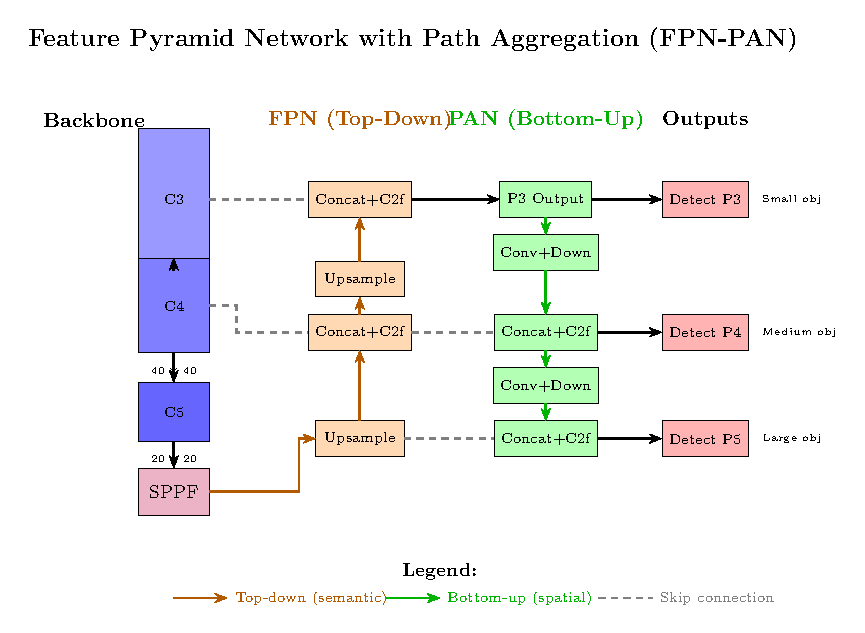
\includegraphics[width=\textwidth]{figures/ch05_fig1_fpn_pan.pdf}
\caption{Feature Pyramid Network with Path Aggregation (FPN-PAN) architecture used in YOLO models. The top-down FPN pathway propagates semantic information from deeper layers to shallower layers through upsampling, while the bottom-up PAN pathway enhances localization signals by propagating spatial information back through the network. Skip connections (dashed lines) enable direct feature reuse across scales. This bidirectional design enables effective multi-scale detection, with P3 features detecting small objects, P4 for medium objects, and P5 for large objects.}
\label{fig:fpn_pan}
\end{figure}

YOLOv5 introduced several training innovations that significantly improved practical usability, including auto-anchor computation that dynamically adjusts anchor box dimensions based on dataset statistics, cosine annealing learning rate scheduling, and comprehensive data augmentation pipelines incorporating mosaic and mixup techniques. The model family spans five size variants ranging from nano to extra-large, with YOLOv5s achieving an mAP of 37.4\% on COCO val2017 at 640 pixel resolution while maintaining inference speeds exceeding 450 frames per second on modern GPU hardware.

\subsection{YOLOv8 Improvements}

YOLOv8, released in January 2023 by Ultralytics, introduced several architectural refinements that address limitations identified in previous versions. The most significant modification involves the transition from a coupled detection head to a decoupled head architecture, separating the classification and localization branches to allow independent optimization of weights for each task. This architectural change typically leads to better convergence during training and improved accuracy, as the network can tune features specifically for identifying what an object is versus determining where it is located.

The backbone architecture in YOLOv8 replaces the C3 modules used in YOLOv5 with the more efficient C2f (Cross-Stage Partial with Two Convolutions and Fusion) module. The C2f design captures richer gradient information by incorporating additional split and concatenation operations, enhancing the model's ability to learn discriminative features while maintaining computational efficiency. This modification proves particularly beneficial when training on synthetic data, where the diversity of rendered appearances requires robust feature extraction capabilities.

\begin{figure}[htbp]
\centering
\begin{tikzpicture}[
    node distance=0.8cm and 1.2cm,
    block/.style={rectangle, draw, fill=blue!20, text width=2.2cm, text centered, minimum height=0.7cm, font=\scriptsize},
    convblock/.style={rectangle, draw, fill=green!20, text width=1.8cm, text centered, minimum height=0.6cm, font=\scriptsize},
    detectblock/.style={rectangle, draw, fill=red!20, text width=1.8cm, text centered, minimum height=0.6cm, font=\scriptsize},
    neckblock/.style={rectangle, draw, fill=orange!20, text width=1.8cm, text centered, minimum height=0.6cm, font=\scriptsize},
    arrow/.style={->, >=stealth, thick},
    dashedarrow/.style={->, >=stealth, thick, dashed}
]

% Backbone
\node[block] (input) {Input\\$640 \times 640 \times 3$};
\node[convblock, below=of input] (conv1) {Conv\\$320 \times 320$};
\node[convblock, below=of conv1] (conv2) {Conv\\$160 \times 160$};
\node[convblock, below=of conv2] (c2f1) {C2f Block\\$160 \times 160$};
\node[convblock, below=of c2f1] (conv3) {Conv\\$80 \times 80$};
\node[convblock, below=of conv3] (c2f2) {C2f Block\\$80 \times 80$};

% Side branch for P3
\node[convblock, right=1.5cm of c2f2] (conv4) {Conv\\$40 \times 40$};
\node[convblock, below=of conv4] (c2f3) {C2f Block\\$40 \times 40$};
\node[convblock, below=of c2f3] (conv5) {Conv\\$20 \times 20$};
\node[convblock, below=of conv5] (c2f4) {C2f Block\\$20 \times 20$};
\node[convblock, below=of c2f4] (sppf) {SPPF\\$20 \times 20$};

% Neck - FPN path
\node[neckblock, left=1.5cm of sppf] (upsample1) {Upsample\\$40 \times 40$};
\node[neckblock, below=of upsample1] (concat1) {Concat + C2f\\$40 \times 40$};
\node[neckblock, below=of concat1] (upsample2) {Upsample\\$80 \times 80$};
\node[neckblock, below=of upsample2] (concat2) {Concat + C2f\\$80 \times 80$};

% PAN path
\node[neckblock, right=1.5cm of concat2] (conv6) {Conv\\$40 \times 40$};
\node[neckblock, below=of conv6] (concat3) {Concat + C2f\\$40 \times 40$};
\node[neckblock, below=of concat3] (conv7) {Conv\\$20 \times 20$};
\node[neckblock, below=of conv7] (concat4) {Concat + C2f\\$20 \times 20$};

% Detection Heads
\node[detectblock, below=0.6cm of concat2] (detect1) {Detect P3\\(Small)};
\node[detectblock, below=0.6cm of concat3] (detect2) {Detect P4\\(Medium)};
\node[detectblock, below=0.6cm of concat4] (detect3) {Detect P5\\(Large)};

% Backbone arrows
\draw[arrow] (input) -- (conv1);
\draw[arrow] (conv1) -- (conv2);
\draw[arrow] (conv2) -- (c2f1);
\draw[arrow] (c2f1) -- (conv3);
\draw[arrow] (conv3) -- (c2f2);
\draw[arrow] (c2f2) -- (conv4);
\draw[arrow] (conv4) -- (c2f3);
\draw[arrow] (c2f3) -- (conv5);
\draw[arrow] (conv5) -- (c2f4);
\draw[arrow] (c2f4) -- (sppf);

% Neck arrows
\draw[arrow] (sppf) -- (upsample1);
\draw[arrow] (upsample1) -- (concat1);
\draw[arrow] (concat1) -- (upsample2);
\draw[arrow] (upsample2) -- (concat2);
\draw[arrow] (concat2) -- (conv6);
\draw[arrow] (conv6) -- (concat3);
\draw[arrow] (concat3) -- (conv7);
\draw[arrow] (conv7) -- (concat4);

% Skip connections
\draw[dashedarrow] (c2f3) -| (concat1);
\draw[dashedarrow] (c2f2) -| (concat2);
\draw[dashedarrow] (concat1) -| (concat3);
\draw[dashedarrow] (sppf) -| (concat4);

% Detection head arrows
\draw[arrow] (concat2) -- (detect1);
\draw[arrow] (concat3) -- (detect2);
\draw[arrow] (concat4) -- (detect3);

% Labels
\node[above=0.1cm of input, font=\small\bfseries] {Backbone};
\node[left=0.1cm of upsample1, font=\small\bfseries, rotate=90, anchor=south] {Neck};
\node[below=0.1cm of detect2, font=\small\bfseries] {Decoupled Heads};

\end{tikzpicture}
\caption{Simplified YOLOv8 architecture showing the backbone with C2f modules, the FPN-PAN neck structure for multi-scale feature fusion, and decoupled detection heads for three output scales. Skip connections (dashed) enable gradient flow and feature reuse across scales.}
\label{fig:yolov8_architecture}
\end{figure}

YOLOv8 also transitions from anchor-based detection to an anchor-free approach, eliminating the need for predefined anchor boxes and simplifying the training pipeline. The anchor-free paradigm directly predicts object centers and dimensions, reducing the number of hyperparameters requiring tuning and improving generalization to objects with aspect ratios not well-represented by predefined anchors. This characteristic proves advantageous when training on synthetic data where object configurations may differ substantially from those in standard benchmark datasets.

\begin{figure}[htbp]
\centering
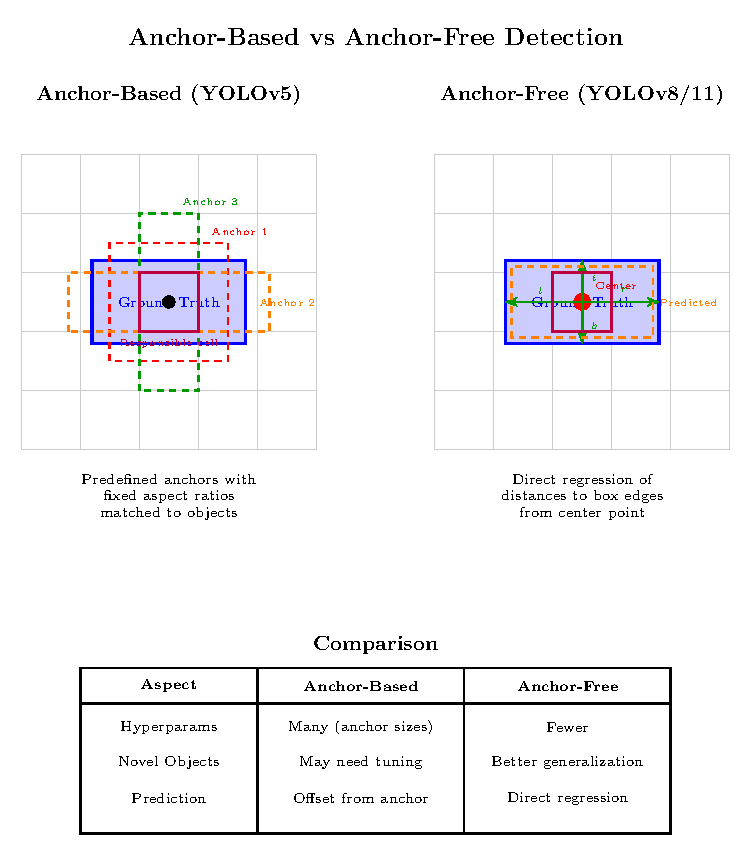
\includegraphics[width=0.95\textwidth]{figures/ch05_fig2_anchor_boxes.pdf}
\caption{Comparison of anchor-based (YOLOv5) and anchor-free (YOLOv8/YOLO11) detection paradigms. In anchor-based detection (left), predefined anchor boxes with various aspect ratios are matched to ground truth objects, and the network predicts offsets from these anchors. In anchor-free detection (right), the network directly regresses distances from the predicted center point to the four box edges ($l$, $r$, $t$, $b$), eliminating the need to predefine anchor dimensions. The anchor-free approach reduces hyperparameters and improves generalization to objects with unusual aspect ratios common in synthetic data.}
\label{fig:anchor_comparison}
\end{figure}

The loss function in YOLOv8 incorporates Distribution Focal Loss (DFL) for bounding box regression, replacing the traditional coordinate regression approach with a distribution-based formulation that models the uncertainty in localization predictions. Combined with Complete Intersection over Union (CIoU) loss for box regression and binary cross-entropy with logits for classification, the composite loss function provides stable training dynamics across diverse data distributions.

\subsection{YOLO11 Latest Features}

YOLO11, released in late 2024, represents the latest stable release in the Ultralytics YOLO family and introduces significant architectural improvements that enhance feature extraction capabilities while optimizing computational graphs. The model architecture refines the C2f module design introduced in YOLOv8, incorporating additional attention mechanisms that improve the network's ability to focus on salient image regions. These attention modules operate with minimal computational overhead, maintaining the real-time inference capabilities expected from YOLO architectures.

The backbone in YOLO11 employs enhanced spatial pyramid pooling with attention (SPPA), extending the traditional SPPF module to incorporate channel and spatial attention mechanisms. This modification improves the model's receptive field coverage while maintaining efficient memory access patterns suitable for deployment on resource-constrained devices. The neck architecture in YOLO11 introduces bi-directional feature pyramid improvements that enhance gradient flow during training, accelerating convergence when training on limited or synthetic datasets.

YOLO11 provides comprehensive task support including object detection, instance segmentation, pose estimation, oriented bounding box detection, and image classification, all within a unified framework. This versatility enables practitioners to experiment with different task formulations when developing synthetic data pipelines, potentially discovering that auxiliary tasks provide useful training signals that improve detection performance. The model maintains backward compatibility with YOLOv8 configuration files while introducing new hyperparameters for controlling the attention mechanism strength and feature fusion strategies.

\subsection{YOLO-NAS and Neural Architecture Search}

YOLO-NAS, developed by Deci AI and released in 2023, represents a fundamentally different approach to YOLO architecture design through the application of Neural Architecture Search (NAS) techniques. Rather than hand-designing architectural components, YOLO-NAS utilizes Deci's proprietary AutoNAC (Automated Neural Architecture Construction) engine to discover optimal block configurations, channel widths, and connectivity patterns for specific hardware targets and accuracy requirements.

The resulting architectures incorporate several innovations not present in manually-designed YOLO variants. YOLO-NAS introduces quantization-aware blocks (QABlocks) that maintain accuracy when the model is converted to INT8 precision through post-training quantization (PTQ). This design consideration proves valuable for edge deployment scenarios where computational resources are limited, but also benefits training pipelines by enabling mixed-precision training without requiring quantization-aware training procedures.

YOLO-NAS achieves notable improvements in small object detection performance, addressing a traditional weakness in YOLO architectures. The NAS-discovered architectures allocate additional capacity to high-resolution feature maps, improving localization accuracy for objects occupying small image regions. Performance benchmarks demonstrate a 20.5\% improvement over YOLOv7, an 11\% improvement over YOLOv5, and a 1.75\% gain compared to YOLOv8 on standard detection benchmarks.

The models come pre-trained on multiple large-scale datasets including COCO, Objects365, and Roboflow 100, providing robust feature representations that transfer effectively to downstream tasks. This extensive pre-training proves particularly valuable for synthetic-to-real transfer scenarios, as the pretrained features encode general object concepts that help bridge the domain gap between synthetic training data and real test environments. However, practitioners should note that Deci was acquired by NVIDIA in 2024, and the original development team no longer actively maintains these models, though Ultralytics continues to provide integration support.

\subsection{Architecture Comparison}

\begin{table}[htbp]
\centering
\caption{Comparison of YOLO Architecture Variants}
\label{tab:yolo_comparison}
\begin{tabular}{p{2.5cm}p{2cm}p{2cm}p{2cm}p{2cm}p{2cm}}
\toprule
\textbf{Feature} & \textbf{YOLOv5} & \textbf{YOLOv8} & \textbf{YOLO11} & \textbf{YOLO-NAS} \\
\midrule
Release Year & 2020 & 2023 & 2024 & 2023 \\
Framework & PyTorch & PyTorch & PyTorch & PyTorch \\
Backbone & CSPDarknet & CSPDarknet (C2f) & CSPDarknet (C2f+Attn) & NAS-optimized \\
Detection Head & Coupled & Decoupled & Decoupled & Decoupled \\
Anchor Type & Anchor-based & Anchor-free & Anchor-free & Anchor-free \\
mAP (COCO) & 50.7\% (v5x) & 53.9\% (v8x) & 54.7\% (11x) & 52.2\% (L) \\
Parameters (S) & 7.2M & 11.2M & 9.4M & 12.2M \\
FPS (A100) & 250 & 280 & 295 & 310 \\
PTQ Support & Limited & No & No & Native \\
Small Object & Baseline & Improved & Enhanced & Best \\
Active Maint. & Yes & Yes & Yes & Limited \\
\bottomrule
\end{tabular}
\end{table}

The architectural comparison presented in Table~\ref{tab:yolo_comparison} highlights the evolutionary trajectory of YOLO designs and the tradeoffs inherent in each variant. For synthetic-to-real training scenarios, several factors warrant particular consideration. The decoupled head architecture present in YOLOv8 and later versions provides faster convergence during fine-tuning, reducing the number of epochs required to achieve stable performance on new data distributions. The anchor-free detection paradigm simplifies training configuration by eliminating the need to tune anchor box dimensions for synthetic data that may contain objects with unusual aspect ratios.

\section{Model Selection for Synthetic Training}
\label{sec:model_selection}

\subsection{Recommendation of YOLOv8s and YOLO11s}

For synthetic-to-real training scenarios where reinforcement learning agents optimize data generation parameters, the small variants of YOLOv8 and YOLO11 (denoted YOLOv8s and YOLO11s) emerge as the recommended choices based on multiple converging factors. These models provide sufficient capacity to learn complex object representations while maintaining training times compatible with iterative optimization loops. The small variants typically require 15-30 minutes per training epoch on modern GPU hardware with datasets of a few thousand images, enabling dozens of training iterations per day within the RL optimization framework.

The YOLOv8s architecture comprises approximately 11.2 million parameters with the C2f backbone and decoupled detection head, achieving an mAP of 44.9\% on COCO val2017 at 640 pixel resolution. This performance level provides a meaningful signal for the RL agent to optimize against while avoiding the overfitting tendencies that larger models exhibit when trained on limited synthetic data. Similarly, YOLO11s offers enhanced feature extraction through its attention mechanisms while maintaining a comparable parameter count, making it suitable for scenarios where improved small object detection is critical.

Research on transfer learning with YOLO architectures demonstrates that models pre-trained on large-scale datasets like COCO significantly outperform scratch-trained models across all evaluation metrics including precision, recall, and mean Average Precision. The pretrained YOLOv8s and YOLO11s models provide feature representations that encode general object concepts, substantially reducing the amount of synthetic data required to achieve acceptable detection performance. This pretraining benefit proves essential when operating within the computational constraints of RL-guided optimization, where training data volume per iteration must remain bounded.

\subsection{Pretrained Backbone Considerations}

The decision to utilize pretrained backbones versus training from scratch fundamentally impacts the synthetic-to-real transfer performance and the efficiency of the overall optimization pipeline. Pretrained backbones, typically initialized with weights learned on the COCO dataset containing 80 object categories and over 200,000 labeled images, provide feature extractors that have learned to identify edges, textures, shapes, and semantic patterns that generalize across visual domains. When fine-tuning on synthetic data, these pretrained features serve as a strong regularization mechanism, constraining the model to representations that transfer well to real images.

The COCO-pretrained weights encode hierarchical visual features ranging from low-level edge detectors in early layers to high-level semantic concept detectors in deeper layers. When the synthetic training data shares similar low-level visual features with real images (common edges, textures, and color distributions), freezing early backbone layers during training preserves these transferable features while allowing later layers to adapt to domain-specific patterns. This selective freezing strategy proves particularly effective when synthetic data exhibits domain shift in high-level appearance characteristics but maintains realistic low-level statistics.

For novel object categories not present in COCO, the pretrained backbone still provides valuable initialization by encoding general feature extraction capabilities. Research demonstrates that pretrained models converge faster and achieve better final performance even when target categories differ entirely from pretraining categories, suggesting that the learned feature representations capture fundamental visual patterns rather than category-specific templates. When training on synthetic data depicting specialized objects, starting from pretrained weights reduces the risk of learning synthetic-specific artifacts that do not transfer to real images.

\subsection{Model Size Tradeoffs}

The YOLO model family provides variants spanning a wide range of computational requirements, from nano models suitable for embedded deployment to extra-large models targeting maximum accuracy. Understanding the tradeoffs between model sizes enables informed selection for synthetic training scenarios where iteration speed and detection performance must be balanced.

Nano variants (YOLOv8n, YOLO11n) containing approximately 3 million parameters offer the fastest training times, typically completing epochs in under 10 minutes on consumer GPU hardware. These models suit exploratory phases of RL optimization where rapid iteration across diverse parameter configurations takes priority over absolute detection accuracy. However, nano models exhibit limited capacity to capture fine-grained appearance variations, potentially providing noisy reward signals that complicate RL agent learning. The shallow feature hierarchies in nano models also show reduced robustness to domain shift, limiting their effectiveness for synthetic-to-real transfer without extensive real data fine-tuning.

Small variants (YOLOv8s, YOLO11s) strike an effective balance between training efficiency and detection capability. With roughly 10 million parameters, these models provide sufficient representational capacity to learn discriminative features from diverse synthetic data while maintaining training times compatible with iterative optimization. Small models demonstrate good transfer learning performance, benefiting substantially from pretrained initialization while remaining adaptable to synthetic domain characteristics.

Medium variants (YOLOv8m, YOLO11m) with approximately 25 million parameters offer improved detection accuracy, particularly for challenging cases involving small objects, occlusion, or unusual viewpoints. The increased capacity enables these models to memorize more training examples, which can be beneficial when synthetic data contains high diversity in object appearances and scene configurations. However, the larger parameter count increases susceptibility to overfitting on limited synthetic data, requiring careful regularization and data augmentation to maintain generalization to real images.

Large and extra-large variants (YOLOv8l/x, YOLO11l/x) containing 40-70 million parameters achieve state-of-the-art accuracy on benchmark datasets but present significant challenges for synthetic training scenarios. Training times increase substantially, reducing the number of iterations possible within RL optimization budgets. More critically, these large models require extensive training data to avoid overfitting, typically exceeding the few thousand images practical for synthetic generation pipelines. Unless real-time inference constraints demand the absolute highest accuracy and computational resources are abundant, practitioners should generally prefer small or medium variants for synthetic-to-real training pipelines.

\subsection{Transfer Learning from COCO}

Transfer learning from COCO-pretrained weights represents the recommended initialization strategy for YOLO models trained on synthetic data. The COCO dataset's diversity encompassing 80 object categories across natural scenes, urban environments, and indoor settings provides feature representations that generalize effectively to most target domains. Research comparing models trained from scratch versus those pre-trained on COCO consistently demonstrates that pretrained models achieve higher accuracy with fewer training epochs, faster convergence, and improved robustness to distribution shift between training and test data.

The transfer learning process involves loading pretrained weights for the backbone and neck components while randomly initializing the detection head layers responsible for category-specific predictions. This partial transfer approach preserves general feature extraction capabilities while allowing the detection head to specialize for target categories present in the synthetic training data. When target categories overlap with COCO categories, practitioners may optionally transfer detection head weights as well, further accelerating convergence and improving final performance.

Fine-tuning pretrained models requires careful learning rate selection to balance adaptation to new data distributions against preservation of transferable features. Research indicates that learning rates approximately 10 times lower than those used for training from scratch provide effective fine-tuning, allowing gradual weight updates that preserve pretrained knowledge while accommodating domain-specific patterns. The cosine annealing learning rate schedule employed by default in YOLO training automatically reduces learning rates during training, providing natural regularization that prevents overfitting to synthetic data characteristics.

\section{Training Configuration for RL Feedback Loops}
\label{sec:training_config}

\begin{figure}[htbp]
\centering
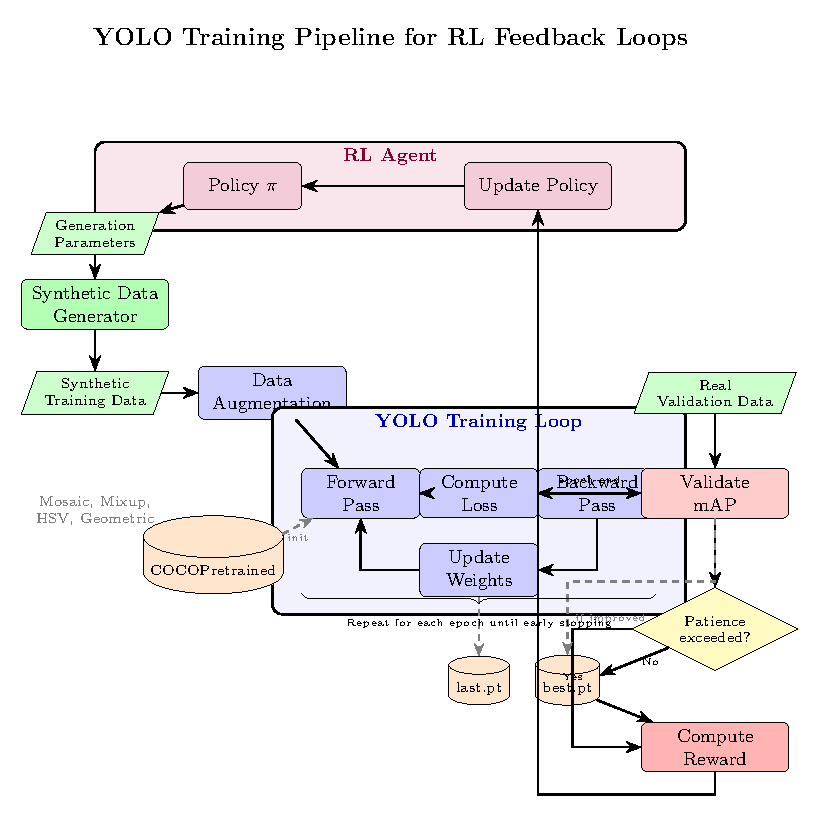
\includegraphics[width=0.95\textwidth]{figures/ch05_fig3_training_pipeline.pdf}
\caption{YOLO training pipeline integrated with reinforcement learning feedback loops for synthetic data optimization. The RL agent's policy generates parameters that control synthetic data generation. Generated training data undergoes augmentation (mosaic, mixup, HSV jittering, geometric transforms) before feeding into the YOLO training loop. Training proceeds with mixed precision (AMP) and early stopping based on validation mAP computed on real images. The best checkpoint (best.pt) is used to compute the reward signal that updates the RL policy, enabling iterative optimization of synthetic data generation parameters.}
\label{fig:training_pipeline}
\end{figure}

\subsection{Hyperparameter Settings for Fast Iteration}

Configuring YOLO training for integration within reinforcement learning feedback loops requires balancing training thoroughness against iteration speed. The RL agent learns to optimize synthetic data generation parameters by observing detection performance on real validation images, necessitating training runs that complete quickly enough to enable meaningful exploration of the parameter space while providing sufficiently accurate performance estimates to guide optimization.

\begin{table}[htbp]
\centering
\caption{Recommended Hyperparameters for RL-Integrated Training}
\label{tab:hyperparameters}
\begin{tabular}{p{3.5cm}p{2.5cm}p{6cm}}
\toprule
\textbf{Parameter} & \textbf{Value} & \textbf{Rationale} \\
\midrule
epochs & 50-100 & Sufficient for convergence with early stopping \\
batch & 16-32 & Balance GPU utilization and gradient noise \\
imgsz & 640 & Standard resolution balancing detail and speed \\
lr0 & 0.01 & Initial learning rate for pretrained models \\
lrf & 0.01 & Final LR ratio for cosine annealing \\
momentum & 0.937 & SGD momentum for stable updates \\
weight\_decay & 0.0005 & L2 regularization against overfitting \\
warmup\_epochs & 3.0 & Gradual LR increase for stability \\
warmup\_momentum & 0.8 & Reduced momentum during warmup \\
box & 7.5 & Box loss gain weighting \\
cls & 0.5 & Classification loss gain \\
dfl & 1.5 & Distribution focal loss gain \\
patience & 20 & Early stopping patience epochs \\
cache & ram & Cache images in RAM for speed \\
amp & True & Enable automatic mixed precision \\
close\_mosaic & 10 & Disable mosaic in final epochs \\
\bottomrule
\end{tabular}
\end{table}

Table~\ref{tab:hyperparameters} presents recommended hyperparameter settings optimized for RL feedback loop integration. The epoch count of 50-100 provides sufficient training duration for models to converge on synthetic data while remaining bounded by early stopping when performance plateaus. Combined with a patience value of 20 epochs, this configuration automatically terminates training when validation metrics cease improving, avoiding wasted computation on converged models.

The learning rate schedule employs cosine annealing from an initial rate of 0.01 to a final ratio of 0.01 (effective final LR of 0.0001), providing gradual learning rate decay that stabilizes training in later epochs. The warmup period of 3 epochs with reduced momentum prevents unstable gradients that can occur when pretrained weights encounter substantially different data distributions, a common occurrence when training on synthetic images with domain shift from COCO.

\subsection{Batch Size Optimization}

Batch size selection significantly impacts both training dynamics and computational efficiency. Larger batch sizes improve GPU utilization by amortizing kernel launch overhead across more samples and provide more stable gradient estimates through reduced sampling variance. However, excessively large batches can reduce model generalization by limiting the exploration of the loss landscape during optimization.

For YOLO training on synthetic data, batch sizes of 16-32 typically provide optimal balance between training speed and model quality. This range maintains sufficient gradient noise to escape local minima while providing stable enough updates for reliable convergence. The batch size also affects batch normalization statistics computed during training; very small batches produce noisy statistics that degrade detection performance, motivating the avoidance of batch sizes below 8 even when GPU memory constraints apply.

The auto-batch feature available in Ultralytics YOLO implementations (specified as batch=-1) automatically determines the largest batch size that fits within available GPU memory, simplifying configuration across different hardware. However, for consistent comparison across RL iterations, fixing the batch size ensures that training dynamics remain comparable, enabling the RL agent to attribute performance differences to data generation parameters rather than training configuration variation.

\subsection{Mixed Precision Training}

Automatic Mixed Precision (AMP) training enables substantial speedups by performing forward and backward passes in FP16 precision while maintaining FP32 master weights for parameter updates. Modern GPU architectures include tensor cores optimized for FP16 matrix operations, achieving 2-8 times higher throughput compared to FP32 computation depending on the specific operation and hardware generation. For YOLO training, AMP typically provides 40-60\% reduction in training time with negligible impact on final model accuracy.

The AMP implementation in PyTorch automatically determines which operations can safely execute in reduced precision while preserving numerical stability for sensitive computations. Loss scaling techniques prevent gradient underflow that can occur when small gradient values fall below FP16 representable range, maintaining training stability across diverse data distributions. For synthetic data training where appearance statistics may differ substantially from typical natural images, the automatic loss scaling in modern AMP implementations proves essential for reliable convergence.

Enabling AMP training requires minimal configuration changes, typically involving only a single boolean flag (amp=True) in YOLO training commands. The computational savings directly translate to increased RL iteration throughput, enabling more extensive exploration of synthetic data generation parameters within fixed time budgets. Given the negligible accuracy impact and substantial speed improvements, AMP should be enabled by default for all RL-integrated training pipelines.

\subsection{Dataset Caching Strategies}

Data loading often constitutes a significant bottleneck in YOLO training pipelines, particularly when training data resides on network storage or mechanical disk drives. Each training iteration requires loading image files, parsing annotation formats, applying augmentation transforms, and transferring data to GPU memory. For RL feedback loops where the same synthetic dataset is used throughout a single training run, caching strategies that preload and retain data in memory can substantially reduce per-epoch training time.

RAM caching (cache='ram') preloads all training images into system memory during the first epoch, eliminating disk I/O for subsequent epochs. This strategy proves highly effective when dataset size fits comfortably within available RAM, typically datasets under 10,000 images with 640x640 resolution consuming approximately 10-15 GB of memory. For the few-thousand image synthetic datasets typical in RL optimization scenarios, RAM caching provides 2-3x speedup in training throughput after the initial loading phase.

Disk caching (cache='disk') creates preprocessed image files in a local cache directory, avoiding repeated decoding and initial preprocessing while maintaining lower memory requirements than RAM caching. This strategy suits scenarios where RAM is constrained but fast local storage is available, such as training on systems with NVMe SSDs. The cache persists across training runs, providing benefits for repeated training on the same synthetic dataset during RL hyperparameter tuning or ablation studies.

For dynamically generated synthetic data where each RL iteration produces new training images, neither caching strategy provides direct benefits since data changes between training runs. However, caching remains valuable during individual training runs when data augmentation creates multiple views of each source image. Practitioners should ensure cache invalidation when synthetic data generation parameters change, avoiding stale cached data that does not reflect current RL agent decisions.

\subsection{Layer Freezing Techniques}

Layer freezing during transfer learning allows practitioners to preserve pretrained features in early network layers while adapting later layers to target domain characteristics. Research on YOLO architectures demonstrates that freezing the first four backbone blocks or the complete backbone can reduce GPU memory usage by up to 28\% while maintaining or improving detection accuracy compared to full fine-tuning. This efficiency gain directly benefits RL feedback loops by reducing per-iteration training time and enabling larger batch sizes within fixed memory budgets.

The effectiveness of layer freezing depends on the relationship between source domain (COCO natural images) and target domain (synthetic rendered images) characteristics. When synthetic data maintains realistic low-level visual features including appropriate edge profiles, texture statistics, and color distributions, freezing early layers preserves effective feature extractors that transfer directly to real test images. Conversely, when synthetic data exhibits substantial low-level distribution shift (e.g., perfect edges without anti-aliasing, unrealistic textures, or limited color variation), freezing early layers can impair adaptation by preventing the network from learning domain-appropriate feature detectors.

The freeze parameter in YOLO training accepts either an integer specifying the number of layers to freeze or a list of layer indices for selective freezing. Setting freeze=10 freezes the first 10 modules (typically the backbone layers) while allowing the neck and head to adapt freely. For synthetic-to-real transfer, starting with backbone freezing and unfreezing layers if validation performance plateaus provides a practical heuristic that reduces training time while maintaining adaptation capability.

Gradual unfreezing strategies offer additional control over the transfer learning process. Beginning training with more layers frozen and progressively unfreezing layers as training progresses allows the network to first adapt high-level features in detection heads before modifying intermediate representations. This approach proves particularly effective when limited real validation data is available to guide training, as it reduces the risk of catastrophic forgetting of pretrained features early in training when optimization signals are noisy.

\begin{algorithm}[htbp]
\caption{YOLO Training Loop with Early Stopping for RL Integration}
\label{alg:training_loop}
\begin{algorithmic}[1]
\Require Synthetic training dataset $\mathcal{D}_{syn}$, Real validation dataset $\mathcal{D}_{val}$
\Require Pretrained model weights $\theta_0$, Maximum epochs $E_{max}$, Patience $P$
\Require Learning rate schedule $\eta(e)$, Loss function $\mathcal{L}$
\Ensure Trained model weights $\theta^*$, Best validation mAP $m^*$

\State Initialize model with pretrained weights: $\theta \leftarrow \theta_0$
\State Initialize best metrics: $m^* \leftarrow 0$, $e^* \leftarrow 0$
\State Initialize early stopping counter: $c \leftarrow 0$
\State Cache training dataset in RAM if memory permits
\State Enable automatic mixed precision (AMP)

\For{epoch $e = 1$ to $E_{max}$}
    \State Set learning rate: $\eta \leftarrow \eta(e)$
    \If{$e > E_{max} - 10$}
        \State Disable mosaic augmentation \Comment{close\_mosaic}
    \EndIf

    \For{each batch $\mathcal{B} \in \mathcal{D}_{syn}$}
        \State Apply augmentation (mosaic, mixup, HSV jitter, geometric)
        \State Forward pass with AMP: $\hat{y} \leftarrow f_\theta(\mathcal{B})$
        \State Compute loss: $L \leftarrow \mathcal{L}(\hat{y}, y)$ \Comment{CIoU + BCE + DFL}
        \State Backward pass with gradient scaling
        \State Update weights: $\theta \leftarrow \theta - \eta \nabla_\theta L$
    \EndFor

    \State Evaluate on validation set: $m \leftarrow \text{mAP}(f_\theta, \mathcal{D}_{val})$

    \If{$m > m^*$}
        \State Update best: $m^* \leftarrow m$, $\theta^* \leftarrow \theta$, $e^* \leftarrow e$
        \State Save checkpoint: best.pt
        \State Reset counter: $c \leftarrow 0$
    \Else
        \State Increment counter: $c \leftarrow c + 1$
    \EndIf

    \If{$c \geq P$}
        \State \textbf{break} \Comment{Early stopping triggered}
    \EndIf
\EndFor

\State \Return $\theta^*$, $m^*$
\end{algorithmic}
\end{algorithm}

\section{Data Augmentation Strategies}
\label{sec:augmentation}

\subsection{Mosaic Augmentation}

Mosaic augmentation, introduced in YOLOv4, represents one of the most impactful data augmentation techniques for object detection training. The technique combines four training images into a single composite image by placing them in a 2x2 grid arrangement with randomized boundaries. This composition forces the model to detect objects in varied contexts, at different relative scales, and with diverse neighboring content, substantially improving generalization to novel scene configurations.

The mosaic technique provides several benefits particularly relevant to synthetic data training. By combining multiple synthetic images, mosaic increases the effective diversity of training batches beyond what the original dataset contains. Objects from different synthetic scenes appear together in novel combinations, reducing the risk that the model learns scene-specific correlations that do not transfer to real images. The technique also exposes the model to objects at smaller relative scales than they appear in original images, improving small object detection performance that often proves challenging in synthetic-to-real transfer.

Mosaic augmentation does introduce potential artifacts that warrant consideration. The artificial boundaries between combined images create discontinuities in scene context that do not occur in natural images. Objects appearing near mosaic boundaries may be partially occluded or placed in impossible spatial relationships with objects from adjacent quadrants. While these artifacts provide useful regularization during early training, they can interfere with learning precise spatial relationships in later training phases. The close\_mosaic parameter addresses this concern by disabling mosaic augmentation during the final epochs (typically 10), allowing the model to refine predictions on unmodified images before evaluation.

\subsection{Mixup and CutMix}

Mixup augmentation extends the linear interpolation concept from classification to object detection by blending pairs of images and their associated labels. Given two images $x_1$ and $x_2$ with corresponding detection targets $y_1$ and $y_2$, mixup creates a composite image $x' = \lambda x_1 + (1-\lambda) x_2$ with combined targets, where the mixing coefficient $\lambda$ is sampled from a Beta distribution. The blended image contains semi-transparent overlays of both source images, forcing the model to detect objects despite reduced visibility and conflicting context.

The mixup probability in YOLO training controls how frequently this augmentation applies, with typical values around 0.1-0.15 providing benefit without excessive training signal noise. Higher mixup probabilities can impair convergence by presenting predominantly blended images that lack the clear object boundaries present in real test images. For synthetic-to-real transfer, moderate mixup helps the model develop robustness to appearance variations while maintaining sensitivity to the distinct object features necessary for accurate detection.

CutMix presents a related but distinct augmentation approach that pastes rectangular patches from one image onto another rather than blending pixel values. The pasted patch brings objects from the source image into novel contexts, increasing effective training diversity. Unlike mixup, CutMix preserves sharp object boundaries within the pasted region while creating artificial boundaries at patch edges. This preservation of local structure may better suit detection tasks where boundary precision impacts localization accuracy.

\subsection{Color Jittering and HSV Augmentation}

Color-based augmentations modify the chromatic appearance of training images to improve model robustness against illumination variation and color distribution shift. The HSV (Hue, Saturation, Value) color space provides intuitive controls for these modifications, allowing independent adjustment of color tone, intensity, and brightness. YOLO training configurations specify HSV augmentation through three parameters controlling the maximum perturbation in each dimension: hsv\_h for hue shift (typically 0.015), hsv\_s for saturation scaling (typically 0.7), and hsv\_v for value scaling (typically 0.4).

For synthetic-to-real transfer, HSV augmentation proves particularly valuable when synthetic rendering produces color distributions that differ from real image statistics. Common rendering artifacts include oversaturated colors, limited dynamic range, and unrealistic lighting that produces uniform illumination without natural gradients. HSV augmentation applied during training exposes the model to broader color variation than present in synthetic data alone, improving generalization to the diverse lighting conditions encountered in real images.

The magnitude of HSV augmentation requires careful tuning for synthetic data scenarios. Excessive color perturbation can create unrealistic training examples that degrade model performance, while insufficient augmentation fails to bridge the color distribution gap between synthetic and real domains. Practitioners should examine representative synthetic images alongside target real images to calibrate appropriate augmentation ranges, ensuring that augmented synthetic images span the color distribution observed in real validation data.

\subsection{Geometric Augmentations}

Geometric augmentations modify the spatial arrangement of image content through transformations including scaling, rotation, translation, shearing, and perspective warping. These augmentations improve model invariance to viewpoint variation and object positioning, critical capabilities for detection tasks where objects appear at diverse orientations and scales.

Scale augmentation (controlled by the scale parameter, typically 0.5) randomly zooms into or out of training images, presenting objects at sizes different from their original capture. This augmentation proves essential when synthetic data generation produces objects at consistent scales that do not match the scale distribution in real test images. Training with scale augmentation ensures the model learns to detect objects across the full range of sizes it will encounter during deployment.

Rotation, translation, and shearing augmentations introduce additional viewpoint variation that complements synthetic data diversity. The degrees parameter controls maximum rotation angle (typically 0.0 for detection to preserve bounding box alignment), while translate (typically 0.1) and shear (typically 0.0) control respective transformation magnitudes. For synthetic-to-real transfer where viewpoint distribution differs between domains, these augmentations help bridge the gap by exposing the model to transformations intermediate between synthetic rendering viewpoints and real image perspectives.

Horizontal flipping (fliplr, typically 0.5) provides viewpoint augmentation with no distortion cost, effectively doubling effective dataset size when objects lack strong lateral asymmetry. Vertical flipping (flipud, typically 0.0 for natural images) applies less frequently as most natural scenes have consistent up-down orientation. These augmentations should match expected real image orientations; training with vertical flips when test images maintain consistent orientation can degrade performance by learning spurious vertical invariance.

\subsection{When to Disable Augmentation}

While data augmentation generally improves model generalization, certain training phases and scenarios benefit from reduced or disabled augmentation. The close\_mosaic parameter in YOLO training automatically disables mosaic augmentation during the final epochs (default 10), allowing the model to refine predictions on unmodified images. This transition removes the artificial context discontinuities introduced by mosaic, enabling more precise localization learning before final evaluation.

For synthetic data training in RL feedback loops, augmentation strategy may vary based on optimization phase. During early RL iterations when exploring diverse data generation parameters, aggressive augmentation helps prevent overfitting to specific synthetic data characteristics. As the RL agent converges toward optimal generation parameters, reduced augmentation allows the detector to learn more precisely from the refined synthetic data, potentially improving the accuracy of reward signals used for final parameter selection.

Validation and test evaluation should always proceed without augmentation to provide consistent performance metrics. The augmented training images do not represent realistic test conditions, and applying augmentation during evaluation would introduce variance that obscures true model capability. YOLO implementations automatically disable augmentation for validation, but practitioners should verify this behavior when using custom evaluation scripts or integrating with RL reward computation.

\section{Loss Functions in YOLO}
\label{sec:loss_functions}

\subsection{Classification Loss}

Classification loss in YOLO architectures measures the accuracy of object category predictions, guiding the network to correctly identify detected objects. Modern YOLO versions employ Binary Cross-Entropy (BCE) loss with logits for multi-label classification, treating each category as an independent binary classification problem. This formulation naturally handles scenarios where a single detection might plausibly belong to multiple related categories, though YOLO datasets typically assign single labels to each ground truth box.

The BCE loss for classification is computed as:
\begin{equation}
\mathcal{L}_{cls} = -\frac{1}{N} \sum_{i=1}^{N} \left[ y_i \log(\sigma(p_i)) + (1-y_i) \log(1-\sigma(p_i)) \right]
\end{equation}
where $N$ is the number of predictions, $y_i$ is the ground truth label, $p_i$ is the predicted logit, and $\sigma$ denotes the sigmoid function. This loss provides strong gradients for both confident incorrect predictions and uncertain correct predictions, driving the model toward high-confidence accurate classifications.

Focal Loss offers an alternative classification loss formulation that addresses class imbalance by down-weighting well-classified examples. The focal loss modifies BCE by multiplying with a modulating factor $(1-p_t)^\gamma$ where $p_t$ is the predicted probability for the correct class and $\gamma$ is a focusing parameter typically set to 2. This modification reduces the loss contribution from easy examples that the model already classifies correctly, focusing learning on hard examples that require additional refinement.

For synthetic-to-real training, the classification loss behavior warrants particular attention. Synthetic data may present object appearances with less variation than real data, leading to overconfident predictions that do not generalize. Monitoring classification confidence calibration on real validation data during training helps identify this issue; if synthetic-trained models produce high-confidence incorrect predictions on real images, increased regularization or focal loss application may improve transfer performance.

\subsection{Localization Loss Evolution}

Bounding box regression loss has evolved substantially across YOLO versions, progressing from simple coordinate regression to sophisticated intersection-based formulations. Early YOLO versions employed Mean Squared Error (MSE) loss on box coordinates, directly penalizing Euclidean distance between predicted and ground truth box parameters. While computationally simple, MSE loss does not directly optimize the evaluation metric (Intersection over Union) and weights coordinate errors independently of their impact on box overlap.

\begin{figure}[htbp]
\centering
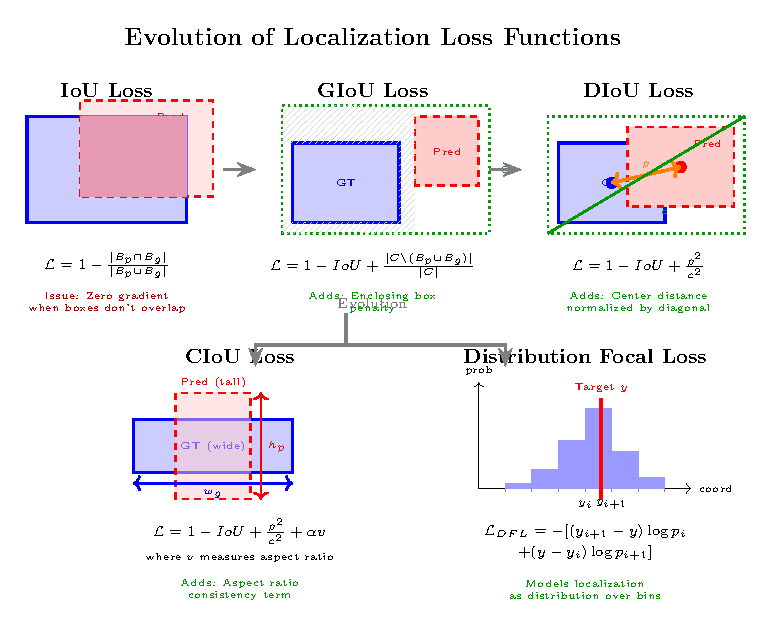
\includegraphics[width=\textwidth]{figures/ch05_fig4_iou_losses.pdf}
\caption{Evolution of localization loss functions in object detection. IoU loss directly optimizes box overlap but provides zero gradients for non-overlapping boxes. GIoU addresses this by penalizing empty space within the enclosing box $C$. DIoU explicitly minimizes center point distance $\rho$ normalized by the diagonal $c$ of the enclosing box. CIoU further adds an aspect ratio consistency term $\alpha v$ to encourage matching box shapes. Distribution Focal Loss (DFL) reformulates coordinate regression as classification over discretized bins, naturally modeling localization uncertainty. Modern YOLO architectures combine CIoU with DFL for robust localization learning.}
\label{fig:iou_losses}
\end{figure}

Intersection over Union (IoU) loss directly optimizes the overlap ratio between predicted and ground truth boxes:
\begin{equation}
\mathcal{L}_{IoU} = 1 - \frac{|B_p \cap B_g|}{|B_p \cup B_g|}
\end{equation}
where $B_p$ and $B_g$ denote predicted and ground truth boxes respectively. IoU loss provides gradients that improve box overlap regardless of the specific coordinate parameterization, but suffers from zero gradient when boxes do not overlap, preventing learning from non-overlapping predictions.

Generalized IoU (GIoU) addresses the non-overlapping gradient issue by incorporating the smallest enclosing box $C$ that contains both prediction and ground truth:
\begin{equation}
\mathcal{L}_{GIoU} = 1 - IoU + \frac{|C \setminus (B_p \cup B_g)|}{|C|}
\end{equation}
The additional term penalizes predictions that, while non-overlapping with ground truth, leave large empty regions within the enclosing box. GIoU provides gradients for all prediction-target pairs regardless of overlap, improving training stability for synthetic data that may produce detection initializations far from ground truth.

Distance IoU (DIoU) explicitly considers the normalized distance between box centers:
\begin{equation}
\mathcal{L}_{DIoU} = 1 - IoU + \frac{\rho^2(b_p, b_g)}{c^2}
\end{equation}
where $\rho(b_p, b_g)$ is the Euclidean distance between predicted and ground truth box centers, and $c$ is the diagonal length of the enclosing box. DIoU provides stronger gradients for center alignment, accelerating convergence compared to GIoU.

\subsection{Complete IoU and Shape-Aware IoU}

Complete IoU (CIoU) extends DIoU by additionally considering aspect ratio consistency between predicted and ground truth boxes:
\begin{equation}
\mathcal{L}_{CIoU} = 1 - IoU + \frac{\rho^2(b_p, b_g)}{c^2} + \alpha v
\end{equation}
where $v$ measures aspect ratio consistency and $\alpha$ is a balancing parameter. The aspect ratio term encourages predictions to match ground truth box shapes, improving localization accuracy for elongated or compact objects. CIoU serves as the default localization loss in YOLOv8 and subsequent versions, providing robust training dynamics across diverse object configurations.

Shape-aware IoU (SIoU) introduces additional terms accounting for angle cost (direction of center displacement), distance cost, and shape cost, providing more comprehensive geometric supervision. SIoU considers the angle between the line connecting box centers and the horizontal axis, encouraging predictions to approach ground truth from geometrically consistent directions. While more complex to compute, SIoU can improve convergence speed and final accuracy for challenging object configurations.

For synthetic-to-real transfer, the choice of localization loss affects how the model interprets box regression errors in synthetic data. CIoU provides a balanced formulation suitable for most scenarios, while SIoU may benefit applications where synthetic data contains objects with distinctive geometric properties (elongated shapes, specific orientations) that should transfer to real detections.

\subsection{Distribution Focal Loss}

Distribution Focal Loss (DFL), introduced in the DAMO-YOLO and incorporated into YOLOv8, reformulates bounding box regression as a classification problem over discretized coordinate distributions. Rather than directly predicting box coordinates, DFL predicts probability distributions over quantized coordinate values, with the final coordinate computed as the expected value of the distribution.

The DFL formulation addresses fundamental limitations of direct coordinate regression. When ground truth coordinates lie between discretization bins, the model must produce a distribution that, in expectation, yields the correct coordinate. This requirement naturally encourages the model to express uncertainty in localization through broader distributions while producing sharp distributions for confidently localized objects.

The DFL is computed as:
\begin{equation}
\mathcal{L}_{DFL} = -[(y_{i+1} - y) \log(p_i) + (y - y_i) \log(p_{i+1})]
\end{equation}
where $y$ is the target coordinate, $y_i$ and $y_{i+1}$ are adjacent discretization points such that $y_i \leq y \leq y_{i+1}$, and $p_i$, $p_{i+1}$ are predicted probabilities for those points. This formulation provides smooth gradients that encourage accurate distribution predictions.

For synthetic data training, DFL offers potential benefits in expressing localization uncertainty. When synthetic objects have appearance features that ambiguously localize boundaries (e.g., simple rendered shapes without detailed textures), the distribution-based formulation allows the model to predict broad distributions reflecting this ambiguity. During real image evaluation, these uncertainty estimates may improve detection reliability by down-weighting ambiguous predictions.

\subsection{Loss Function Configuration}

The composite loss function in YOLO combines classification, localization, and distribution losses with configurable weighting:
\begin{equation}
\mathcal{L}_{total} = \lambda_{box} \mathcal{L}_{CIoU} + \lambda_{cls} \mathcal{L}_{BCE} + \lambda_{dfl} \mathcal{L}_{DFL}
\end{equation}
where $\lambda_{box}$, $\lambda_{cls}$, and $\lambda_{dfl}$ control the relative importance of each component. Default YOLOv8 values of 7.5, 0.5, and 1.5 respectively emphasize localization accuracy while maintaining sufficient classification and distribution learning signals.

Adjusting loss weights can tune model behavior for specific synthetic-to-real transfer requirements. Increasing the classification weight $\lambda_{cls}$ encourages the model to focus on discriminating between object categories, beneficial when synthetic data contains objects with ambiguous appearances that might be confused. Reducing the box weight $\lambda_{box}$ may help when synthetic object boundaries differ systematically from real object boundaries, allowing the model to learn classification features more strongly while treating localization as secondary.

\section{Early Stopping and Convergence}
\label{sec:early_stopping}

\subsection{Patience-Based Early Stopping}

Early stopping provides automatic training termination when model performance on held-out validation data ceases to improve. The patience parameter specifies the number of consecutive epochs without improvement that triggers training termination. For YOLO training, patience values of 20-50 epochs typically provide appropriate balance between avoiding premature termination during temporary performance plateaus and preventing excessive computation after convergence.

The early stopping criterion monitors the primary validation metric, typically mAP@0.5 (mean Average Precision at IoU threshold 0.5) or mAP@0.5:0.95 (averaged across IoU thresholds from 0.5 to 0.95). When synthetic data characteristics differ substantially from real validation data, the validation mAP trajectory may exhibit more variability than typical same-domain training, motivating slightly increased patience values to distinguish genuine convergence from noisy performance fluctuations.

Implementation of early stopping requires maintaining the best-performing model checkpoint throughout training. Each time validation performance improves, the current model weights save to disk (typically as best.pt) and the patience counter resets. When patience epochs pass without improvement, training terminates and the best checkpoint provides the final model. This checkpoint-based approach ensures that the returned model represents peak validation performance even if training continued past the optimal epoch.

\subsection{Validation Frequency Optimization}

The frequency of validation evaluation impacts both training throughput and early stopping sensitivity. Default YOLO configurations evaluate validation performance after each training epoch, providing fine-grained monitoring of learning progress. However, each validation pass incurs computational overhead that extends total training time, particularly for large validation sets or complex evaluation metrics.

For RL feedback loops where training iteration speed is critical, reducing validation frequency can accelerate training while maintaining meaningful early stopping behavior. Evaluating every 5 or 10 epochs rather than every epoch reduces validation overhead proportionally while still capturing the general trajectory of performance improvement. The tradeoff involves potentially continuing training slightly past the optimal stopping point when the best epoch falls between validation evaluations.

The small real validation sets (approximately 50 images) typical in synthetic-to-real scenarios enable rapid validation evaluation, often completing in seconds compared to minutes-long training epochs. In these scenarios, per-epoch validation provides negligible overhead while maximizing the precision of early stopping decisions. Practitioners should profile validation time relative to epoch duration to inform frequency optimization decisions.

\subsection{Checkpoint Strategies}

Checkpoint management strategies determine which model states persist during training and how storage resources allocate across the training run. YOLO training by default maintains two checkpoint files: last.pt containing the most recent epoch's weights, and best.pt containing the weights from the epoch achieving highest validation performance. This dual-checkpoint approach ensures access to both the convergence endpoint and the peak-performance state.

For RL integration, the best.pt checkpoint provides the natural model state for reward computation, as it represents the maximum detection capability achieved during training on the current synthetic data. Computing RL rewards based on best.pt performance rather than final epoch performance ensures that temporary training instabilities or overfitting in later epochs do not corrupt the reward signal used for synthetic data optimization.

Extended checkpoint histories recording weights from multiple epochs enable post-hoc analysis of training dynamics and alternative model selection criteria. Saving checkpoints every N epochs creates a trajectory of model states that can inform understanding of how synthetic data characteristics influence learning progress. However, the storage requirements for extensive checkpoint histories can become substantial for large models, motivating selective checkpoint retention based on validation performance milestones.

Resume functionality allows training to continue from saved checkpoints, enabling recovery from interruptions and extension of training beyond initial epoch budgets. When RL optimization identifies promising synthetic data configurations, extended training from checkpoints can refine detection performance beyond what initial training epochs achieved. The resume capability requires preserving optimizer state alongside model weights, ensuring consistent learning rate scheduling and momentum accumulation across resumed training sessions.

\section{Practical Considerations for Reinforcement Learning Integration}

The integration of YOLO training within reinforcement learning optimization loops introduces considerations beyond standalone model development. The training pipeline must support automated execution without manual intervention, produce consistent and comparable results across iterations, and complete within time budgets compatible with meaningful parameter space exploration.

Deterministic training through fixed random seeds enables reproducible results that isolate the impact of synthetic data parameter changes from training stochasticity. Setting seeds for Python random number generation, NumPy, and PyTorch (including CUDA operations) provides reproducibility that strengthens the correlation between RL agent parameter choices and observed detection performance. However, some GPU operations remain non-deterministic even with fixed seeds, introducing residual variance that the RL algorithm must accommodate.

Automated metric logging and structured result storage facilitate RL agent access to training outcomes. YOLO training produces comprehensive logs including per-epoch loss values, validation metrics, and training configuration details. Integrating these logs with RL experiment tracking enables analysis of how synthetic data parameters influence training dynamics, potentially revealing relationships useful for warm-starting RL optimization or constraining parameter search spaces.

Hardware resource management ensures consistent training throughput across RL iterations. GPU memory allocation, data loading workers, and CPU utilization should remain stable across training runs to prevent variable iteration times that complicate RL scheduling. Containerized training environments provide isolation that maintains resource consistency regardless of system background activity.

\section{Summary}

This chapter has presented a comprehensive examination of YOLO architecture evolution and training strategies optimized for synthetic-to-real domain adaptation scenarios. The progression from YOLOv5 through YOLOv8 and YOLO11 demonstrates continuous refinement of feature extraction, detection head design, and loss function formulation that improves both accuracy and training efficiency. The small model variants, particularly YOLOv8s and YOLO11s, emerge as recommended choices for RL-guided synthetic data optimization, balancing detection capability against iteration speed requirements.

Training configuration for RL feedback loops requires careful attention to hyperparameter selection, mixed precision training, caching strategies, and layer freezing techniques that collectively determine iteration throughput. Data augmentation strategies including mosaic, mixup, and HSV jittering expand effective training diversity while the close\_mosaic mechanism ensures refined final-epoch learning on unmodified images.

The evolution of loss functions from simple coordinate regression through GIoU, DIoU, CIoU, and Distribution Focal Loss reflects deepening understanding of localization supervision requirements. Early stopping with appropriate patience values and checkpoint management enables efficient training termination while preserving peak-performance model states for RL reward computation.

Together, these architectural choices and training strategies form a comprehensive framework for deploying YOLO detectors within reinforcement learning systems that optimize synthetic data generation for real-world object detection applications.
